% Takze podkapitola by sa mohla napr. volat "Klasifikacna metoda Random Forests".

% V podkapitole chces popisat nasledujuce veci:
% - Preco si si vybral prave tuto klasifikacnu metodu (lepsie zdovodnenie ako "je mi sympaticka")
% - V strucnosti popisat, ako funguje klasifikator (algoritmus trenovania a klasifikacie), ake su jeho vystupy (cislo na intervale [0,1] a co take cislo znamena)
% - Popisat metody vyhodnocovania uspesnosti a akym sposobom sa meria "dolezitost atributov"

Ako klasifikátor sme si vybrali \textit{náhodný les (angl. Random forest)}, pretože patrí v~súčasnosti medzi najlepšie klasifikátory. V~tejto sekcii si popíšeme základný algoritmus a v~čom spčívajú jeho vyhody a jeho najdôležitejšie vlastnosti.


\subsubsection[Dôležité vlastnosti]{Dôležité vlastnosti náhodných lesov}
Klasifikátor náhodný les má niekoľko dôležitých vlastností, kvôli ktorým sme si ho vybrali:
\begin{itemize}
\item má vysokú presnosť (podľa \cite{randomForest} je najpresnejší spomedzi všetkých vtedajších klasifikačných algoritmov)
\item je efektívny aj na veľkých dátach
\item dokáže obsiahnuť tisícky vstupných premenných
\item natrénovaný náhoný les môžme uložiť a neskôr použiť na ďalšie dáta
\item dáva odhad, ktoré premenné sú dôležité na klasifikáciu.
\end{itemize}

Navyše má ešte niekoľko ďaľších užitočných vlastností, ktoré však pre nás neboli rozhodujúce:

\begin{itemize}
\item dokáže sa vysporiadať aj s~väčším množstvom chýbajúcich dát
\item produkuje interný nevychýlený odhad chyby aj počas trénovania lesa
\item dokáže počítať vzťahy medzi atribútmi a klasifikáciou
\item počíta vzdialenosť medzi jednotlivími pármi prípadov, čo môže byť použité pri clusteringu a detekcii outlierov alebo ponúknuť zaujímavé pohľady na dáta.
\item počítanie vzdialenosti môže byť použité aj na neoanotované\footnote{bez informácie o~triede} dáta, čo sa dá použiť na klastrovanie, detekciu outlierov.
\item Ponúka experimentálnu metódu na detekciu interakcie medzi premennými.
\end{itemize}

\subsection{Klasifikačné stromy}
Keďže náhodný les je vlastne les \textit{klasifikačných stromov \footnote{niekedy označované ako rozhodovacie stromy}}, je nevyhnutné, aby sme si najskôr povedali niečo o~nich.

%subsection?
Klasifikačný strom je strom vybudovaný na základe trénovacej množiny, ktorý na základe vstupných údajov (vstupného vektora) predpovedá hodnotu výstupnej premennej. Klasifikačný strom sa skladá z~\textit{uzlov} a \textit{listov}. V~uzle sa nachádza rozdeľovacie kritérium, podľa ktorého sa vieme rozhodnúť do ktorej vetvy máme pokračovať. V~listoch sa nachádzajú triedy, do ktorých sa vstupný vektor klasifikuje.


\begin{figure}[htp]
    \centering
    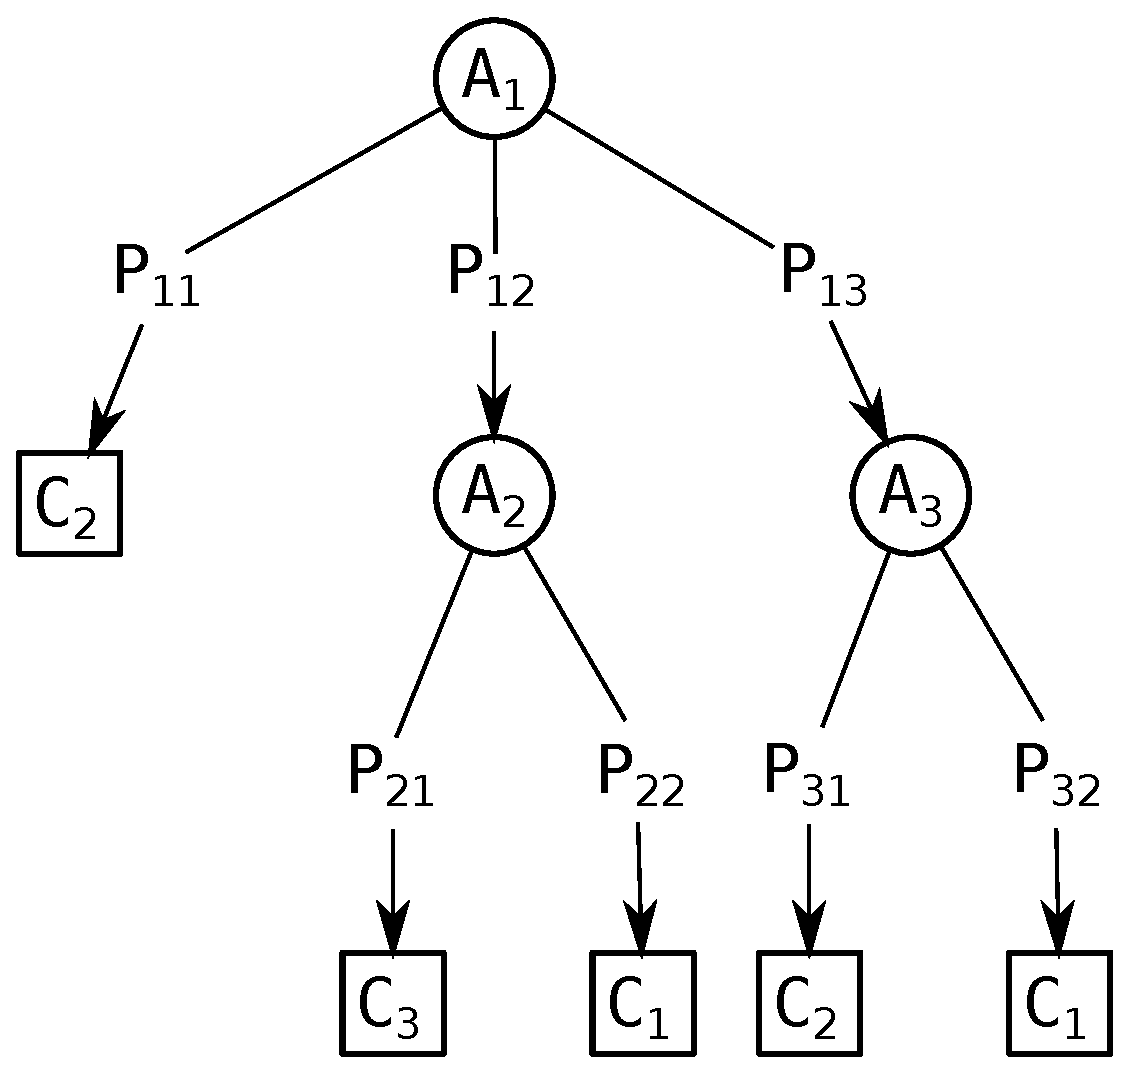
\includegraphics[width=.5\textwidth]{images/decision_tree}
    \caption[Klasifikačný strom]{Klasifikačný strom. $A$ sú atribúty, $P$ sú konkrétne hodnoty atribútov a $C$ sú triedy, do ktorých klasifikujeme dáta.}
\end{figure}

Klasifikácia vstupného vektora vyzerá nasledovne: prechádzame strom zhora nadol a postupne sa zaraďujeme do vetiev podľa rozdelovacích kritérií. Podľa toho, v~ktorom liste skončíme, sa určí výstupná hodnota.

\subsubsection{Trénovanie}

Na trénovanie rozdovacích stromov sa používajú rôzne algoritmy. My si spomenieme najjednoduchší z~nich -- algoritmus ID3 \cite{wiki:id3}. Budeme rozlišovať dva typy listov: uzavretý a neuzavretý list. Uzavreté listy majú už priradenú triedu. Neuzavreté listy ešte nemajú priradenú triedu. Ku každému neuzavretému list prislúcha nejaká sada príkladov.

Algoritmus začína so stromom, ktorý má práve jeden vrchol -- neuzavretý list. Kým existuje nejaký neuzavretý list $l$ opakuje:
\begin{itemize}
    \item Ak sú v~jednom liste všetky príklady jednej triedy, označí list touto triedou a získame uzavretý list.
    \item Inak vyberie najinformatívnejší atribút $A_l$ a vrcholu $l$ pridá deti, rozdelené podľa hodnôt atribútu $A_l$.
\end{itemize}

Najinformatívnejší atribút vyberáme pomocou miery \textit{zisk informácie (angl. information gain)}. Zisk informácie je založený na rozdieli entrópie pred a po rozdelení podľa daného atribútu. Nech $C$ je množina tried a $p_c$ je pravdepodobnosť, že náhodný prvok z~$S$ patrí do $C$, potom entropiu množiny $S$ počítame ako:
$$E(S) = -\sum_{c \in C} p_c\log{p_c}$$
Zisk informácie potom vypočítame takto:
$$IG(S,A) = E(S) - \sum_{v \in A} \frac{\left| S_{\{A=v\}} \right|}{\left| S \right|} E\left(S_{\{A=v\}}\right)$$

\subsection{Náhodný les}

\subsubsection{Klasifikácia}
Náhodný les sa skladá z~mnohých klasifikačných stromov, ktoré tvoria komisiu. Pri klasifikácii nejakého vstupného vektora sa predloží vstupný vektor každému stromu. Každý strom následne vráti klasifikáciu a hovoríme, že stromy \textit{hlasujú}. Náhodný les následne zvolí klasifikáciu podľa väčšiny z~hlasov všetkých stromov v~lese.

%TODO parametrizacia rf

\subsubsection{Trénovanie}

Pri trénovaní náhodných lesov sa využívajú dve hlavné techniky. Prvou z~nich je takzvaný \textit{bagging}, alebo tiež \textit{bootstrapping}. Máme $N$ trénovacích vektorov. Trénovaciu množinu pripravíme pre každý strom zvlášť tak, že z~pôvodných $N$ vektorov vyberieme náhodne s~opakovaním $N$ vektorov, ktoré budú použité na natrénovanie daného rozhodovacieho stromu.

Druhá technika spočiva v~zmene trénovacieho algoritmu pre stromy. Nech trénovacie vektory majú $M$ atribútov. Namiesto všetkých $M$ atribútov sa v~každom vrchole vyberie náhodne len $m<<M$ z~nich. Najlepší atribút na rozdelenie vrcholu sa potom vyberá z~týchto $m$ atribútov, pričom $m$ je konštantné počas celého algoritmu.

Každý strom je potom plne natrenovaný, bez orezávania.

Parameter $m$ je jediným parametrom, na ktorý je náhodný les citlivý. Ako bolo ukázané v~\cite{randomForestPaper}, chyba náhodného lesu závisí na dvoch veciach: korelácii medzi dvoma storomami v~lese (zvýšenie korelácie vedie k~zväčšeniu chyby) a sily\footnote{silný klasifikátor je taký, ktorý má malú chybu} každého stromu v~lese (zvýšenie sily jednotlivých stromov vedie k~zníženiu chyby). Ak znížime $m$ znížime oboje -- koreláciu aj silu stromov. Optimálny rozsah $m$ je zvyčajne celkom veľký a v~praxi sa zvykne často používať $m = \sqrt{M}$ alebo sa zvykne $m$ zvoliť tak aby sa minimalizovala \textit{out of bag}\footnote{dáta, ktoré sa nenachádzajú v~jednotlivých trénovacích množinách pre dané stromy, viac v~\cite{randomForest}} chyba.



